% Options for packages loaded elsewhere
\PassOptionsToPackage{unicode}{hyperref}
\PassOptionsToPackage{hyphens}{url}
%
\documentclass[
  man]{apa6}
\usepackage{amsmath,amssymb}
\usepackage{iftex}
\ifPDFTeX
  \usepackage[T1]{fontenc}
  \usepackage[utf8]{inputenc}
  \usepackage{textcomp} % provide euro and other symbols
\else % if luatex or xetex
  \usepackage{unicode-math} % this also loads fontspec
  \defaultfontfeatures{Scale=MatchLowercase}
  \defaultfontfeatures[\rmfamily]{Ligatures=TeX,Scale=1}
\fi
\usepackage{lmodern}
\ifPDFTeX\else
  % xetex/luatex font selection
\fi
% Use upquote if available, for straight quotes in verbatim environments
\IfFileExists{upquote.sty}{\usepackage{upquote}}{}
\IfFileExists{microtype.sty}{% use microtype if available
  \usepackage[]{microtype}
  \UseMicrotypeSet[protrusion]{basicmath} % disable protrusion for tt fonts
}{}
\makeatletter
\@ifundefined{KOMAClassName}{% if non-KOMA class
  \IfFileExists{parskip.sty}{%
    \usepackage{parskip}
  }{% else
    \setlength{\parindent}{0pt}
    \setlength{\parskip}{6pt plus 2pt minus 1pt}}
}{% if KOMA class
  \KOMAoptions{parskip=half}}
\makeatother
\usepackage{xcolor}
\usepackage{graphicx}
\makeatletter
\def\maxwidth{\ifdim\Gin@nat@width>\linewidth\linewidth\else\Gin@nat@width\fi}
\def\maxheight{\ifdim\Gin@nat@height>\textheight\textheight\else\Gin@nat@height\fi}
\makeatother
% Scale images if necessary, so that they will not overflow the page
% margins by default, and it is still possible to overwrite the defaults
% using explicit options in \includegraphics[width, height, ...]{}
\setkeys{Gin}{width=\maxwidth,height=\maxheight,keepaspectratio}
% Set default figure placement to htbp
\makeatletter
\def\fps@figure{htbp}
\makeatother
\setlength{\emergencystretch}{3em} % prevent overfull lines
\providecommand{\tightlist}{%
  \setlength{\itemsep}{0pt}\setlength{\parskip}{0pt}}
\setcounter{secnumdepth}{-\maxdimen} % remove section numbering
% Make \paragraph and \subparagraph free-standing
\ifx\paragraph\undefined\else
  \let\oldparagraph\paragraph
  \renewcommand{\paragraph}[1]{\oldparagraph{#1}\mbox{}}
\fi
\ifx\subparagraph\undefined\else
  \let\oldsubparagraph\subparagraph
  \renewcommand{\subparagraph}[1]{\oldsubparagraph{#1}\mbox{}}
\fi
\newlength{\cslhangindent}
\setlength{\cslhangindent}{1.5em}
\newlength{\csllabelwidth}
\setlength{\csllabelwidth}{3em}
\newlength{\cslentryspacingunit} % times entry-spacing
\setlength{\cslentryspacingunit}{\parskip}
\newenvironment{CSLReferences}[2] % #1 hanging-ident, #2 entry spacing
 {% don't indent paragraphs
  \setlength{\parindent}{0pt}
  % turn on hanging indent if param 1 is 1
  \ifodd #1
  \let\oldpar\par
  \def\par{\hangindent=\cslhangindent\oldpar}
  \fi
  % set entry spacing
  \setlength{\parskip}{#2\cslentryspacingunit}
 }%
 {}
\usepackage{calc}
\newcommand{\CSLBlock}[1]{#1\hfill\break}
\newcommand{\CSLLeftMargin}[1]{\parbox[t]{\csllabelwidth}{#1}}
\newcommand{\CSLRightInline}[1]{\parbox[t]{\linewidth - \csllabelwidth}{#1}\break}
\newcommand{\CSLIndent}[1]{\hspace{\cslhangindent}#1}
\ifLuaTeX
\usepackage[bidi=basic]{babel}
\else
\usepackage[bidi=default]{babel}
\fi
\babelprovide[main,import]{english}
% get rid of language-specific shorthands (see #6817):
\let\LanguageShortHands\languageshorthands
\def\languageshorthands#1{}
% Manuscript styling
\usepackage{upgreek}
\captionsetup{font=singlespacing,justification=justified}

% Table formatting
\usepackage{longtable}
\usepackage{lscape}
% \usepackage[counterclockwise]{rotating}   % Landscape page setup for large tables
\usepackage{multirow}		% Table styling
\usepackage{tabularx}		% Control Column width
\usepackage[flushleft]{threeparttable}	% Allows for three part tables with a specified notes section
\usepackage{threeparttablex}            % Lets threeparttable work with longtable

% Create new environments so endfloat can handle them
% \newenvironment{ltable}
%   {\begin{landscape}\centering\begin{threeparttable}}
%   {\end{threeparttable}\end{landscape}}
\newenvironment{lltable}{\begin{landscape}\centering\begin{ThreePartTable}}{\end{ThreePartTable}\end{landscape}}

% Enables adjusting longtable caption width to table width
% Solution found at http://golatex.de/longtable-mit-caption-so-breit-wie-die-tabelle-t15767.html
\makeatletter
\newcommand\LastLTentrywidth{1em}
\newlength\longtablewidth
\setlength{\longtablewidth}{1in}
\newcommand{\getlongtablewidth}{\begingroup \ifcsname LT@\roman{LT@tables}\endcsname \global\longtablewidth=0pt \renewcommand{\LT@entry}[2]{\global\advance\longtablewidth by ##2\relax\gdef\LastLTentrywidth{##2}}\@nameuse{LT@\roman{LT@tables}} \fi \endgroup}

% \setlength{\parindent}{0.5in}
% \setlength{\parskip}{0pt plus 0pt minus 0pt}

% Overwrite redefinition of paragraph and subparagraph by the default LaTeX template
% See https://github.com/crsh/papaja/issues/292
\makeatletter
\renewcommand{\paragraph}{\@startsection{paragraph}{4}{\parindent}%
  {0\baselineskip \@plus 0.2ex \@minus 0.2ex}%
  {-1em}%
  {\normalfont\normalsize\bfseries\itshape\typesectitle}}

\renewcommand{\subparagraph}[1]{\@startsection{subparagraph}{5}{1em}%
  {0\baselineskip \@plus 0.2ex \@minus 0.2ex}%
  {-\z@\relax}%
  {\normalfont\normalsize\itshape\hspace{\parindent}{#1}\textit{\addperi}}{\relax}}
\makeatother

\makeatletter
\usepackage{etoolbox}
\patchcmd{\maketitle}
  {\section{\normalfont\normalsize\abstractname}}
  {\section*{\normalfont\normalsize\abstractname}}
  {}{\typeout{Failed to patch abstract.}}
\patchcmd{\maketitle}
  {\section{\protect\normalfont{\@title}}}
  {\section*{\protect\normalfont{\@title}}}
  {}{\typeout{Failed to patch title.}}
\makeatother

\usepackage{xpatch}
\makeatletter
\xapptocmd\appendix
  {\xapptocmd\section
    {\addcontentsline{toc}{section}{\appendixname\ifoneappendix\else~\theappendix\fi\\: #1}}
    {}{\InnerPatchFailed}%
  }
{}{\PatchFailed}
\keywords{keywords\newline\indent Word count: X}
\DeclareDelayedFloatFlavor{ThreePartTable}{table}
\DeclareDelayedFloatFlavor{lltable}{table}
\DeclareDelayedFloatFlavor*{longtable}{table}
\makeatletter
\renewcommand{\efloat@iwrite}[1]{\immediate\expandafter\protected@write\csname efloat@post#1\endcsname{}}
\makeatother
\usepackage{lineno}

\linenumbers
\usepackage{csquotes}
\usepackage{tabu}
\usepackage{tikz}
\usepackage{adjustbox}
\usepackage{float}
\usepackage{graphicx}
\usepackage{pdflscape}
\usepackage{lscape}
\usepackage{longtable}
\usepackage{tabu}
\usepackage{setspace}% http://ctan.org/pkg/setspace
\AtBeginEnvironment{longtable}{\singlespacing}{\small}
\ifLuaTeX
  \usepackage{selnolig}  % disable illegal ligatures
\fi
\IfFileExists{bookmark.sty}{\usepackage{bookmark}}{\usepackage{hyperref}}
\IfFileExists{xurl.sty}{\usepackage{xurl}}{} % add URL line breaks if available
\urlstyle{same}
\hypersetup{
  pdftitle={Estimating age-related change in infants' linguistic and cognitive development using (meta-)meta-analysis},
  pdfauthor={Anjie Cao1, Molly Lewis2, Sho Tsuji3, Christina Bergmann4, Alejandrina Cristia3, \& Michael C. Frank1},
  pdflang={en-EN},
  pdfkeywords={keywords},
  hidelinks,
  pdfcreator={LaTeX via pandoc}}

\title{Estimating age-related change in infants' linguistic and cognitive development using (meta-)meta-analysis}
\author{Anjie Cao\textsuperscript{1}, Molly Lewis\textsuperscript{2}, Sho Tsuji\textsuperscript{3}, Christina Bergmann\textsuperscript{4}, Alejandrina Cristia\textsuperscript{3}, \& Michael C. Frank\textsuperscript{1}}
\date{}


\shorttitle{Estimating change with meta-analysis}

\authornote{

Enter author note here.

Correspondence concerning this article should be addressed to Anjie Cao, 450 Jane Stanford Way, Stanford, CA 94305. E-mail: \href{mailto:anjiecao@stanford.edu}{\nolinkurl{anjiecao@stanford.edu}}

}

\affiliation{\vspace{0.5cm}\textsuperscript{1} Stanford University\\\textsuperscript{2} Carnegie Mellon University\\\textsuperscript{3} École Normale Supérieure - PSL\\\textsuperscript{4} Hochschule Osnabrück}

\abstract{%
Developmental psychology focuses on how psychological phenomena emerge with age. In cognitive development research, however, the specifics of this emergence is often underspecified. Researchers often provisionally assume linear growth by including chronological age as a predictor in regression models. In this work, we aim to evaluate this assumption by examining the functional form of age trajectories across 24 phenomena in early linguistic and cognitive development using (meta-)meta-analysis. Surprisingly, for most meta-analyses, the effect size for the phenomenon was relatively constant throughout development. We investigated four possible hypotheses explaining this pattern: (1) age-related selection bias against younger infants; (2) methodological adaptation for older infants; (3) change in only a subset of conditions; and (4) positive growth only after infancy. None of these explained the lack of age-related growth in most datasets. Our work challenges the assumption of linear growth in early cognitive development and suggests the importance of uniform measurement across children of different ages.
}



\begin{document}
\maketitle

Developmental psychology focuses on how psychological constructs change with age. Throughout the years, many theories have been proposed to characterize and explain how and why developmental changes happen (Bronfenbrenner, 1977; Carey, 2009; Elman, 1996; Flavell, 1994; e.g., Piaget, 1971; Thelen \& Smith, 2007). Among these theories, one common assumption is that skills increase with age (positive change assumption): children get better as they get older. Often, researchers treat age as a predictor in linear regression models, and therefore implicitly assume that the constructs of interests follow a linear trajectory (Lindenberger \& Pötter, 1998). While both assumptions are widely adopted, especially in early cognitive and language development, their validity is rarely tested.

One common approach to evaluating the functional form of age-related changes is through longitudinal studies. Measurements of psychological constructs, when tracked longitudinally, often reveal age trajectories that violate the linearity assumption. For instance, a longitudinal study that follows the development of executive function (EF) from 3 to 5 years-old using a battery of EF tasks show that EF follows a non-linear trajectory over age (Johansson, Marciszko, Brocki, \& Bohlin, 2016). Similarly, vocabulary in early childhood, measured by MacArthur-Bates Communicative Development Inventories, also follows the exponential trend rather than the linear trend (Frank, Braginsky, Yurovsky, \& Marchman, 2021). In many domains with established measurements, longitudinal research has been used to characterize the functional form of the development (Adolph, Robinson, Young, \& Gill-Alvarez, 2008; Cole, Lougheed, Chow, \& Ram, 2020; Karlberg, Engström, Karlberg, \& Fryer, 1987; McArdle, Grimm, Hamagami, Bowles, \& Meredith, 2009; Tilling, Macdonald-Wallis, Lawlor, Hughes, \& Howe, 2014). However, longitudinal methods are more rarely applied to experimental studies that identify proposed mechanisms underlying development.

Many important findings in early language and cognitive development are primarily attested in cross-sectional experimental studies. For example, in the language learning domain, many studies have targeted specific mechanisms proposed to underlie how infants acquire specific facets of language. Constructs such as mutual exclusivity (Markman \& Wachtel, 1988), statistical learning (Saffran, Aslin, \& Newport, 1996), syntactic bootstrapping (Naigles, 1990) and so on, are all attested through decades of experimental evidence acquired through cross-sectional studies. These works are critical to test the causal mechanisms underlying age-related changes, but they are rarely measured in samples with sufficient size and age variation to test the positive change assumption or the assumption of linearity (cf. Frank et al., 2017). In an ideal world, one would run those experiments longitudinally on a large, diverse sample. In practice, this goal is difficult to achieve due to the constraints on both time and financial resources. As a result, the functional forms of age-related changes in critical constructs remain poorly understood.

To address this issue, we turned to meta-analysis. Meta-analysis is a statistical method to aggregate evidence across studies quantitatively. This approach has been widely adopted in many disciplines and subfields, including developmental psychology (Doebel \& Zelazo, 2015; e.g. Hyde, 1984; Letourneau, Duffett-Leger, Levac, Watson, \& Young-Morris, 2013). Compared to the single study approach, meta-analysis has several advantages. First, it allows us to examine the robustness of the phenomena documented in the literature. By combining results from multiple studies, meta-analysis enhances the statistical power to detect effects that might be too small to identify in individual studies. Second, meta-analysis provides a framework for assessing the consistency of research findings across different contexts (Borenstein, Hedges, Higgins, \& Rothstein, 2021; Egger, Smith, \& Phillips, 1997). Further, pooling across developmental studies with different cross-sectional samples may yield sufficient variation to explore the functional form of age-related change with greater precision than individual studies.

In this work, we aim to leverage meta-analysis to examine the shape of the developmental trajectory in key constructs in infant language and cognitive development. Specifically, we use existing meta-analyses from Metalab (\url{https://langcog.github.io/metalab/}), a platform that hosts community-augmented meta-analyses. Metalab was established to provide dynamic databases publicly available to all researchers (Bergmann et al., 2018). Researchers can deposit their meta-analysis dataset in the platform, and they can also use the dataset for custom analyses (e.g. Cao, Lewis, \& Frank, 2023; Lewis et al., 2016). To this date, Metalab contains 2967 effect sizes from 32 different meta-analysis, spanning different areas of developmental psychology. This resource allows us to examine the suitability of meta-analysis as a tool to characterize developmental trajectory -- and if suitable, provides insights into how these key constructs develop across the early months of childhood.

We acknowledge at the outset that meta-analysis has significant limitations. The quality of a meta-analysis is necessarily constrained by the quality of the existing studies (Simonsohn, Simmons, \& Nelson, 2022). If the studies being aggregated are flawed, the conclusions drawn from the meta-analysis will also be questionable. Moreover, one significant issue in interpreting meta-analysis is the heterogeneity among studies. Heterogeneity refers to the variability in study participants, interventions, outcomes, and methodologies. This diversity can make it challenging to aggregate results meaningfully, because differences between studies may reflect true variation in effects rather than a singular underlying effect size (Fletcher, 2007; Higgins \& Thompson, 2002; Huedo-Medina, Sánchez-Meca, Marı́n-Martı́nez, \& Botella, 2006; Thompson \& Sharp, 1999). Critically, understanding the source of heterogeneity often requires detailed coding of the potential moderators; this process is frequently hampered by the inadequate reporting standards prevalent in psychological literature, which often leaves essential information for coding these moderators absent (Nicholson, Deboeck, \& Howard, 2017; Publications \& Journal Article Reporting Standards., 2008). In other words, whether meta-analysis can provide insights into the nature of age-related change is dependent upon the quality of the existing literature.

This paper is organized as follows. In the first section, we provide an overview on the estimated general shape of age-related change across the datasets in Metalab. To preview our findings, we found that most datasets showed relatively constant effect size across age. This finding challenges the commonly held linearity assumption and the positive increase assumption. In the second section, we test four hypotheses on why the current meta-analyses failed to reveal age-related changes: (1) age-related selection bias against younger infants; (2) methodological adaptation for older infants; (3) change in only a subset of conditions; and (4) positive growth only after infancy. We found that none of the four explanations provided a satisfying explanation for the lack of age-related change in most meta-analyses.

\begin{lltable}

\begin{longtable}{llllll}\noalign{\getlongtablewidth\global\LTcapwidth=\longtablewidth}
\caption{\label{tab:unnamed-chunk-12} This table summarizes the number of effect sizes (ES) and the number of participants included in each dataset. The ES estimates represent the aggregated effect sizes and their 95\% confidence intervals. The $I^2$ measures the heterogneity of each dataset. The paper source column indicates the published record associated with each dataset.}\\
\toprule
Dataset & \multicolumn{1}{c}{N ES} & \multicolumn{1}{c}{N Subject} & \multicolumn{1}{c}{MA ES} & \multicolumn{1}{c}{$I^2$} & \multicolumn{1}{c}{Source paper}\\
\midrule
\endfirsthead
\caption*{\normalfont{Table \ref{tab:unnamed-chunk-12} continued}}\\
\toprule
Dataset & \multicolumn{1}{c}{N ES} & \multicolumn{1}{c}{N Subject} & \multicolumn{1}{c}{MA ES} & \multicolumn{1}{c}{$I^2$} & \multicolumn{1}{c}{Source paper}\\
\midrule
\endhead
Abstract rule learning & 95 & 1123 & 0.22 [0.07, 0.37] & 0.80 & Rabagliati et al., (2018)\\
Audio-visual congruence & 92 & 4132 & 0.33 [0.19, 0.47] & 0.89 & Cox et al., (2022)\\
Categorization bias & 80 & 594 & 0.16 [-0.66, 0.99] & 0.96 & NA\\
Cross-situational word learning & 48 & 2241 & 0.67 [0.5, 0.84] & 0.90 & NA\\
Familiar word recognition & 34 & 586 & 0.54 [0.38, 0.69] & 0.55 & Carbajal et al., (2021)\\
Gaze following (combined) & 81 & 1407 & 0.81 [0.61, 1.01] & 0.90 & Frank et al., (2016)\\
Infant directed speech preference & 100 & 1267 & 0.37 [0.25, 0.49] & 0.71 & Zettersten et al., (2023)\\
Label advantage in concept learning & 100 & 1644 & 0.36 [0.23, 0.48] & 0.73 & NA\\
Language discrimination & 104 & 1479 & -0.26 [-0.4, -0.11] & 0.77 & Gasparini et al., (2021)\\
Language preference & 49 & 641 & 0.11 [-0.06, 0.28] & 0.93 & Gasparini et al., (2021)\\
Mispronunciation sensitivity & 249 & 2122 & 0.45 [0.24, 0.66] & 0.94 & Von Holzen \& Bergmann (2021)\\
Mutual exclusivity & 131 & 2222 & 1.27 [0.99, 1.56] & 0.95 & Lewis et al. (2020)\\
Natural speech preference & 55 & 786 & 0.44 [0.23, 0.65] & 0.83 & Issard et al., (2023)\\
Neonatal Imitation & 336 & 2455 & 0.68 [0.4, 0.97] & 0.94 & Davis et al. (2021)\\
Online word recognition & 14 & 330 & 1.37 [0.78, 1.96] & 0.95 & Frank et al., (2016)\\
Prosocial agents & 61 & 1244 & 0.4 [0.29, 0.52] & 0.20 & Margoni \& Surian (2018)\\
Simple arithmetic competences & 14 & 369 & 0.25 [0.04, 0.46] & 0.54 & Christodoulou et al., (2017)\\
Sound symbolism & 44 & 425 & 0.16 [-0.01, 0.33] & 0.69 & Fort et al. (2018)\\
Statistical sound category learning & 20 & 591 & 0.29 [0.01, 0.57] & 0.58 & Cristia (2018)\\
Statistical word segmentation & 103 & 804 & -0.08 [-0.18, 0.02] & 0.83 & Black \& Bergmann (2017)\\
Switch task & 143 & 2764 & -0.16 [-0.25, -0.06] & 0.78 & Tsui et al., (2019)\\
Syntactic bootstrapping & 60 & 832 & 0.24 [0.03, 0.44] & 0.72 & Cao \& Lewis (2022)\\
Vowel discrimination (native) & 143 & 2418 & 0.59 [0.43, 0.75] & 0.78 & Tsuji \& Cristia (2014)\\
Vowel discrimination (non-native) & 49 & 600 & 0.65 [0.2, 1.1] & 0.92 & Tsuji \& Cristia (2014)\\
Word segmentation (combined) & 315 & 2910 & 0.2 [0.14, 0.26] & 0.78 & Bergmann \& Cristia (2016)\\
\bottomrule
\end{longtable}

\end{lltable}

\begin{table*}[hbt]
\ifnextchar[{\eatarg}{}
[tbp]

\begin{center}
\begin{threeparttable}

\caption{\label{tab:unnamed-chunk-10} This table summarizes the values of $\Delta$ of corrected Akaike Information Criterion (AICc) for the age model with different functional forms: Constant, Linear, Logarithmic, and Quadratic. The values were calculated from subtracting the minimum AICc from the AICc of each model. They were rounded to two decimal. The bold values indicate the best fitting model. Asterisks indicate models that are a significantly better fit compared to other functional forms for that dataset.}

\begin{tabular}{lllll}
\toprule
Dataset & \multicolumn{1}{c}{Const} & \multicolumn{1}{c}{Linear} & \multicolumn{1}{c}{Log} & \multicolumn{1}{c}{Quadratic}\\
\midrule
Cross-situational word learning & \bf{0.00} & 2.44 & 2.29 & 2.55\\
Language discrimination & \bf{0.00} & 1.32 & 0.91 & 1.59\\
Prosocial agents & \bf{0.00} & 2.08 & 1.87 & 2.15\\
Simple arithmetic competences & \bf{0.00*} & 6.65* & 6.74* & 6.55*\\
Statistical word segmentation & \bf{0.00} & 1.34 & 1.51 & 1.12\\
Switch task & \bf{0.00} & 1.12 & 1.15 & 1.06\\
Syntactic bootstrapping & \bf{0.00} & 0.71 & 0.56 & 0.88\\
Vowel discrimination (native) & \bf{0.00} & 1.34 & 0.99 & 1.63\\
Vowel discrimination (non-native) & \bf{0.00} & 1.56 & 1.67 & 1.46\\
Word segmentation (combined) & \bf{0.00} & 1.28 & 1.05 & 1.61\\
Infant directed speech preference & \bf{0.00} & 1.57 & 1.47 & 1.53\\
Mispronunciation sensitivity & 1.89 & \bf{0.00} & 0.05 & 0.19\\
Online word recognition & 2.22 & \bf{0.00} & 0.23 & 0.15\\
Sound symbolism & 3.91 & \bf{0.00} & 0.61 & 0.09\\
Audio-visual congruence & 5.90* & 6.70* & \bf{0.00*} & 7.44*\\
Label advantage in concept learning & 2.37 & 0.95 & \bf{0.00} & 1.63\\
Mutual exclusivity & 9.80* & 0.58 & \bf{0.00*} & 1.38\\
Neonatal Imitation & 2.25 & 0.36 & \bf{0.00} & 1.06\\
Abstract rule learning & 0.44 & 0.32 & 0.86 & \bf{0.00}\\
Categorization bias & 8.46* & 0.62 & 1.36 & \bf{0.00*}\\
Familiar word recognition & 1.68 & 0.28 & 1.15 & \bf{0.00}\\
Gaze following (combined) & 43.73* & 2.07 & 10.41* & \bf{0.00*}\\
Language preference & 2.50 & 2.36 & 4.12 & \bf{0.00}\\
Natural speech preference & 0.86 & 0.43 & 1.04 & \bf{0.00}\\
Statistical sound category learning & 3.44 & 1.04 & 3.01 & \bf{0.00}\\
\bottomrule
\end{tabular}

\end{threeparttable}
\end{center}

\end{table*}
\efloatseparator

\hypertarget{estimating-the-functional-forms-of-the-developmental-change-in-meta-analytic-data}{%
\section{Estimating the functional forms of the developmental change in meta-analytic data}\label{estimating-the-functional-forms-of-the-developmental-change-in-meta-analytic-data}}

\hypertarget{datasets}{%
\subsection{Datasets}\label{datasets}}

Datasets were retrieved from Metalab. As of February 2024, Metalab hosted 32 datasets in total, with research areas ranging from language learning to cognitive development. All datasets included effect size estimates converted to standardized mean difference (SMD; also known as Cohen's \emph{d}) as well as estimates of effect size variance and a variety of other moderators (e.g., average age of participants) provided by the contributors. There were 2 desiderata for the datasets to be included in the final analysis:

\begin{enumerate}
\def\labelenumi{\arabic{enumi}.}
\tightlist
\item
  The dataset must describe an experimental (non-correlational) effect that uses behavioral measures, and
\item
  For a dataset that has already been published, the meta-analytic effect reported in the published form must not be null (i.e., must be significantly different than zero).
\end{enumerate}

Five datasets did not meet the first desideratum (\emph{Pointing and vocabulary (concurrent)}; \emph{Pointing and vocabulary (longitudinal)}; \emph{Video deficit}; \emph{Symbolic play}; \emph{Word segmentation (neuro)}), and one dataset did not meet the second desideratum (\emph{Phonotactic learning}). These datasets were not included in the analysis.

For the remaining 26 datasets, we made the following modifications. Following the organization in the original meta-analysis (Gasparini, Langus, Tsuji, \& Boll-Avetisyan, 2021), we separated the \emph{Language discrimination and preference} dataset into two datasets, one for discrimination and one for preference. We also combined two pairs of datasets because they were testing the same experimental effects: \emph{Gaze following (live)} and \emph{Gaze following (video)} was combined into \emph{Gaze following (combined)}; \emph{Function word segmentation} and \emph{Word segmentation (behavioral)} was combined into \emph{Word segmentation (combined)}. We also replaced the \emph{Infant directed speech preference} dataset with a more up-to-date version reported in Zettersten et al. (2023).

To make the comparison more equivalent to each other, we would run models with the same random effect structure specifications across all datasets. To achieve this goal, we recoded the relevant grouping variables in the datasets with missing grouping variables.

Since we were mostly interested in the age trajectory of these constructs in early childhood, we further trimmed the datasets to include only effect sizes from participants under 36 months of age. This decision did not qualitatively affect our findings as most datasets did not include data above age 36 months. The final analysis included 25 datasets in total. Table 1 presented the names of all the datasets, along with the number of effect sizes and participants included for each dataset.

\hypertarget{methods}{%
\subsection{Methods}\label{methods}}

All of the statistical analyses were conducted in R. Meta-analytic models were fit using the \texttt{metafor} package (Viechtbauer, 2010). This was an exploratory study in which no hypotheses were pre-registered.

For each dataset, we considered four functional forms as possible candidates for the shape of the developmental trajectory: linear, logarithmic, quadratic, and constant. A linear form is the most common assumption in the literature, whereas logarithmic and quadratic were chosen to represent sublinear growth and superlinear growth, respectively. The constant form served as a baseline null hypothesis for the other alternative growth patterns. Although other, more complex growth patterns are of course possible, we opted to compare these forms as a first pass. Note that the constant model includes one parameter (an intercept), linear and logarithmic models include two parameters (an intercept and a slope), and the quadratic model includes three parameters (intercept, slope, and quadratic growth term).

For all analyses, we fit multilevel random-effects meta-regression models using nested random intercepts to account for both the testing of individual samples in multiple conditions (e.g., in a between-participants design) and multiple studies within a single paper. Meta-regression models predicted effect sizes (standardized mean difference / Cohen's d) with mean age in months in different functional forms. We fit four meta-regression models in total for each dataset.

\hypertarget{results}{%
\subsection{Results}\label{results}}

\hypertarget{model-comparison}{%
\subsubsection{Model comparison}\label{model-comparison}}

Our initial goal was to compare the fit of models with different functional forms for each meta-analysis. Because models differed in their complexity (number of parameters), we extracted the corrected AIC (AICc) for each model. The model with the lowest AICc was considered the baseline model, and all the remaining models were compared against the baseline. The remaining model each received a \(\Delta_{AIC}\), which was the difference between the AIC of the model and the AIC of the baseline model. Following statistical convention, we treated \(\Delta_{AIC} > 4\) as the statistical significance threshold (Burnham \& Anderson, 2004). A baseline model was significantly better than an alternative model if and only if the alternative model had \(\Delta_{AIC} > 4\).

Surprisingly, the four functional forms could not be meaningfully distinguished in 19 out of 25 datasets.. (This situation typically arises because the data are constant and hence more complex models with zero parameters fit the data equally well \footnote{In the situation of a completely constant pattern of effects across age, the maximal difference in model fit would be an AICc of exactly 4 between the constant and quadratic model, reflecting a two-parameter difference.}). The remaining 6 datasets yielded meaningful contrasts between different functional forms, but the linear form was not the best-fitting form for any dataset. Table 2 shows the model comparison results for each dataset. Figure 1 shows the prediction of each functional form.

\hypertarget{linearity-and-positive-increase-assumption}{%
\subsubsection{Linearity and Positive Increase Assumption}\label{linearity-and-positive-increase-assumption}}

One limitation of the model comparison approach is that it does not quantify growth over time. To further examine the positive increase assumption, we estimated linear meta-regression models and examined the estimates on the age predictor. We found that the slope estimate for age was not significantly different from zero the in majority of the datasets (16/25; Figure 2).

\hypertarget{discussion}{%
\subsection{Discussion}\label{discussion}}

We conducted model comparisons to assess the functional forms of age-related change across 25 datasets. Four functional forms---Logarithmic, Linear, Quadratic, and Constant---were largely indistinguishable within most datasets. Notably, in datasets where contrasts were meaningful, linear models received no support, challenging the prevalent linearity assumption for early linguistic and cognitive development. Further, we only detected any positive growth in 8/25 meta-analyses. Past work has successfully revealed age-related changes using meta-analysis (e.g. Best \& Charness, 2015; McCartney, Harris, \& Bernieri, 1990; Sugden \& Marquis, 2017). But in most datasets that we have considered, effect size does not increase with age. Why?

\begin{figure}
\centering
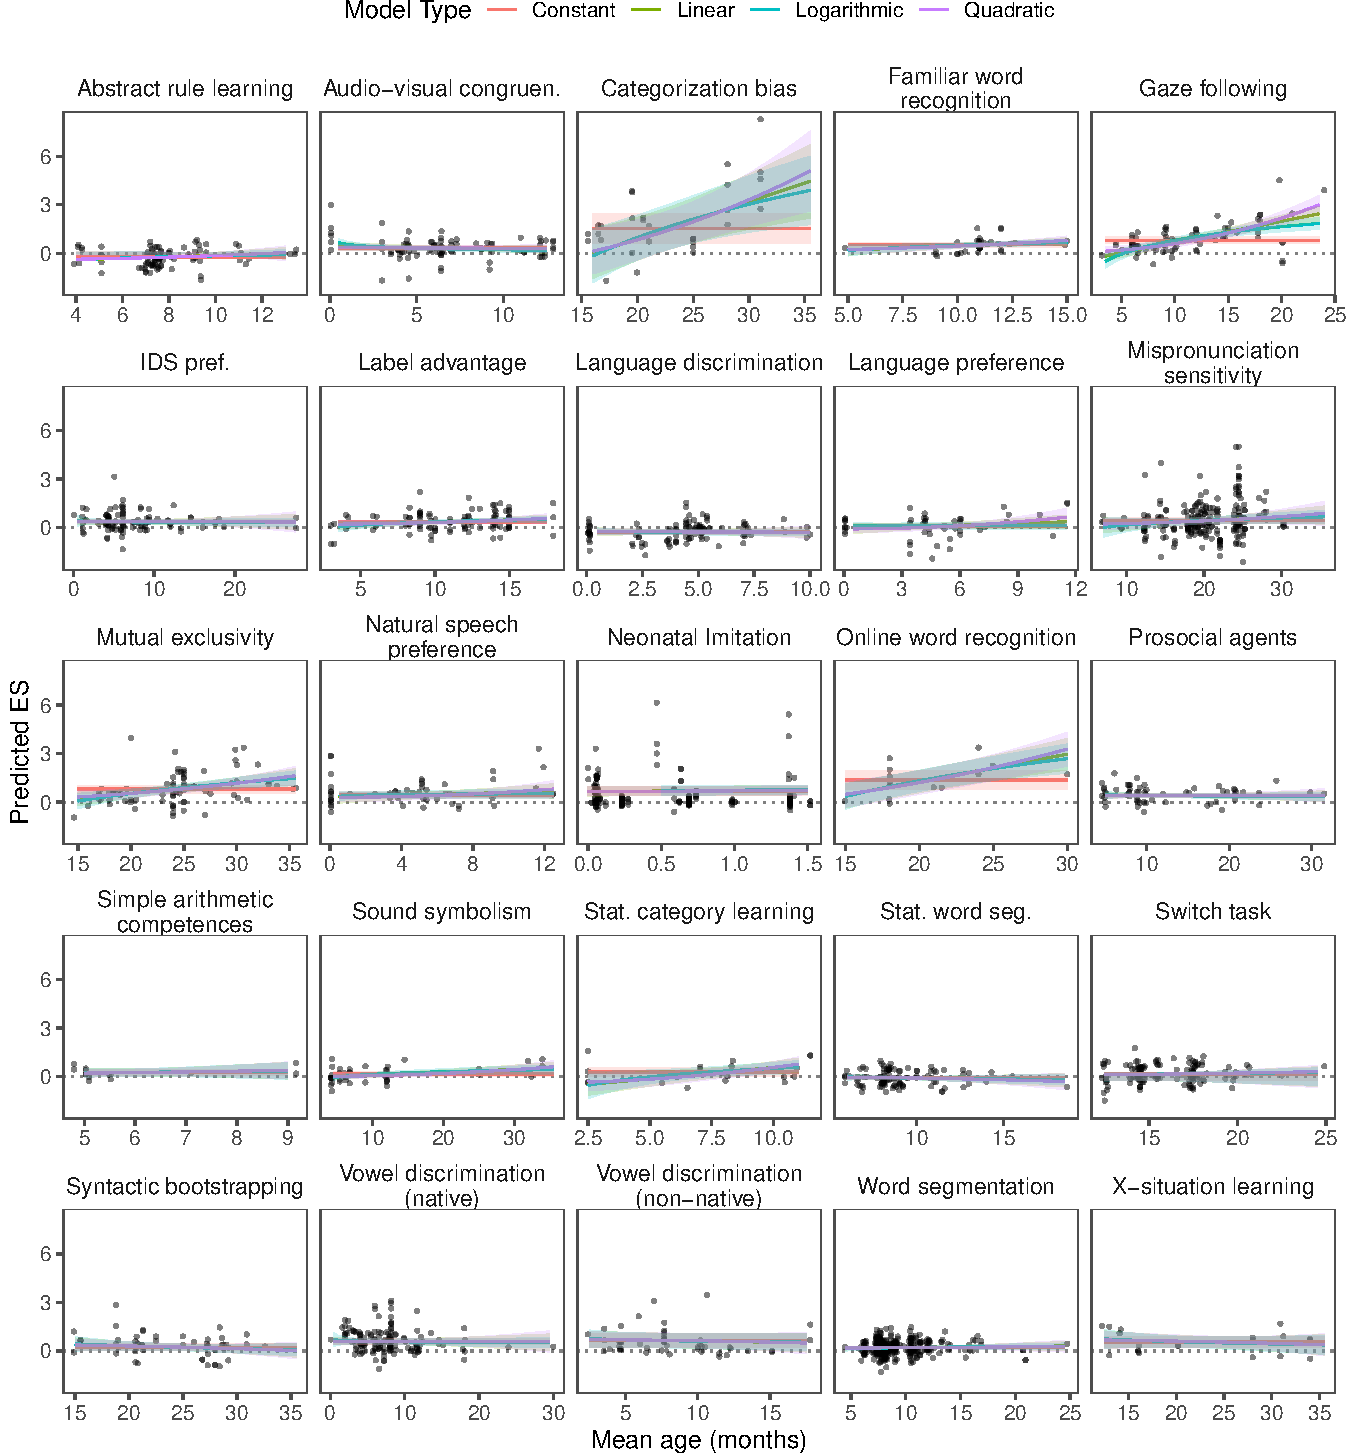
\includegraphics{00_main_files/figure-latex/unnamed-chunk-19-1.pdf}
\caption{\label{fig:unnamed-chunk-19}Each panel shows the dataset and the predicted values of the four functional forms. For each panel, X-axis represent the age in month, and Y-axis represents the effect size. The shaded area is the 95\% confidence interval of the prediction.}
\end{figure}

\begin{figure}
\centering
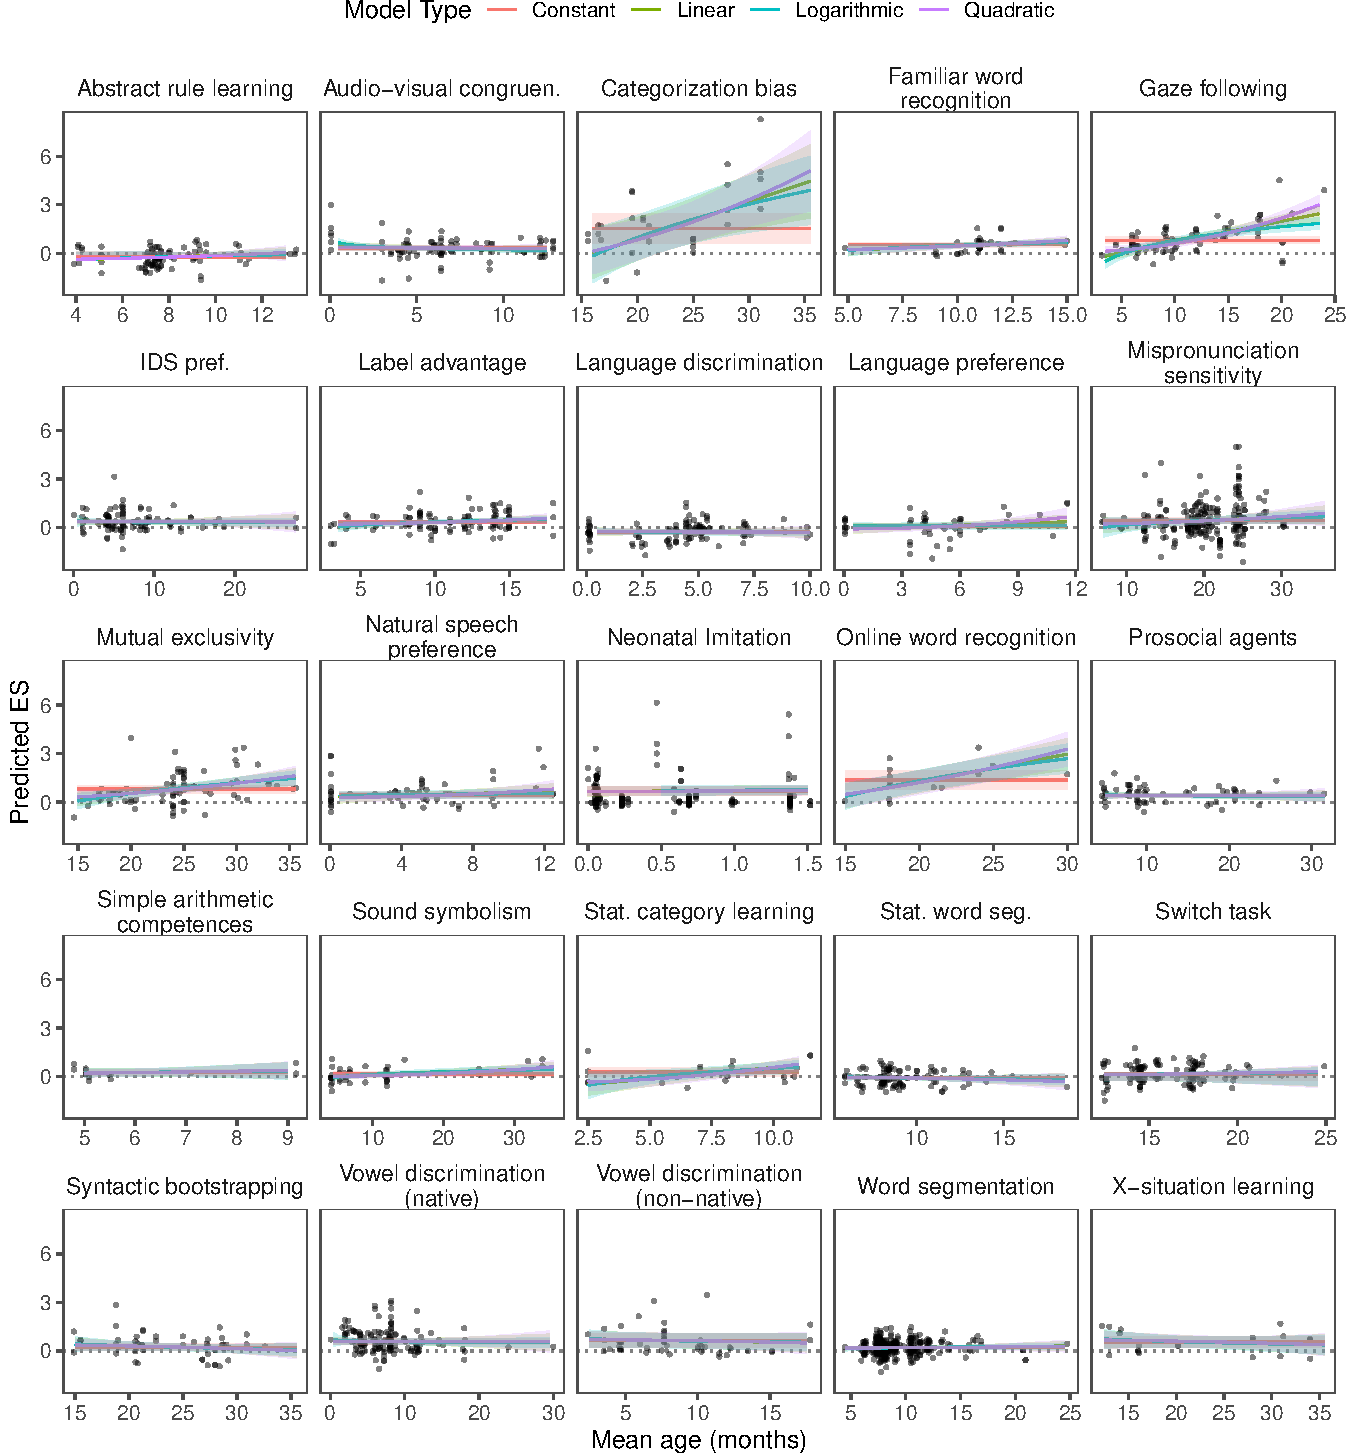
\includegraphics{00_main_files/figure-latex/unnamed-chunk-20-1.pdf}
\caption{\label{fig:unnamed-chunk-20}Each dot represents the estimate of the age predictor in the linear model. Red dots indicate the particular estimate is statistically significant, and black indicate the estimate is not significant. Error bars show 95\% confidence intervals.}
\end{figure}

Here we consider four explanations for the lack of age-related change in most of the meta-analyses we examined. First, meta-analyses are susceptible to publication bias (Ferguson \& Brannick, 2012; Ferguson \& Heene, 2012; Francis, 2012; Thornton \& Lee, 2000). And the bias could be related to the characteristics of the study, such as the inclusion of younger participants (Kathleen M. Coburn \& Vevea, 2015). Consequently, studies with younger participants may have effect sizes that were more inflated, compared to the studies with older participants. The selectivity of publication bias would thus obscure the possible developmental changes in the dataset (Figure 3, Panel 1).

Second, researchers may change methods as infants expand their behavioral repertoire (Figure 3, Panel 2). For example, the high-amplitude sucking paradigm is most likely to be deployed on very young infants, whereas the looking paradigm is most likely to be used on older infants. We did see some evidence for method adaptation in some datasets. For example, in \emph{Language discrimination}, the average age for studies using a sucking paradigm was 0.58 months (SD = 0.89), but 5.30 months (SD = 1.78) for studies using looking time paradigm. This age-related change in research paradigms could lead to a case of Simpson's paradox: the age-related trend within a single method might be lost when multiple methods are combined (Kievit, Frankenhuis, Waldorp, \& Borsboom, 2013; Simpson, 1951).

Third, other methodological factors unrelated to age could also contribute to the lack of developmental effects. 22 of the 25 datasets included in the current analyses has a manuscript associated. Among the manuscripts, 8 identified that the meta-analytic effects were only robust in a subset of the studies. Some of the subsets were identified by certain methodological characters (e.g.~in \emph{Syntactic Bootstrapping}, the effect was only present in studies with transitive conditions, Cao \& Lewis, 2022), and other subsets were identified by participants characteristics (e.g.~in \emph{Familiar word recognition}, the effect was stronger in infants whose primary language exposure was from Romance languages, Carbajal, Peperkamp, \& Tsuji, 2021). Perhaps the apparent lack of developmental effects in the current analysis could be attributed to a complex interaction between methodological factors and participant characteristics, rather than a true absence of developmental changes (Figure 3, Panel 3).

Fourth, developmental change in infancy and early childhood might be distinct from one another. Bergelson (2020) has speculated that word comprehension in the looking-while-listening paradigm only shows significant developmental changes after 12 months of age, with infants younger than 12 months showing mostly flat developmental trajectories in this task. This contrast could be attributed to the fact that older infants are not only more experienced compared to younger infants, but also better learners who can more effectively take advantage of the input they receive. Could this pattern generalize to other tasks and domains? There is much evidence suggesting that developmental changes occurring in one domain would have cumulative, cascading effects on changes in other domains (Ahmed, Kuhfeld, Watts, Davis-Kean, \& Vandell, 2021; Bornstein, Hahn, Putnick, \& Pearson, 2018; Oakes \& Rakison, 2019). The outcome of such developmental cascades might not be measurable in the experimental tasks included in the meta-analyses until infants are above 12 months of age (Figure 3, Panel 4).

We investigate each of these explanations in turn, assessing empirical support in our data. We summarise the results of these analyses in Table 3; in brief, no explanation provided traction for more than a small number of datasets.

\def\checkmark{\tikz\fill[scale=0.4](0,.35) -- (.25,0) -- (1,.7) -- (.25,.15) -- cycle;}

\begin{lltable}

\begin{longtable}{lllllll}\noalign{\getlongtablewidth\global\LTcapwidth=\longtablewidth}
\caption{\label{tab:unnamed-chunk-12} This table presents whether the original dataset shows any evidence for linear growth, and to what extent there is evidence supporting the four hypotheses (Checkmarks for yes, crosses for no). Absence of any symbol suggests that there is not enough data to test the hypothesis.}\\
\toprule
\multicolumn{1}{c}{Dataset} & \multicolumn{1}{c}{Linear Growth} & \multicolumn{2}{c}{H1} & \multicolumn{1}{c}{H2} & \multicolumn{1}{c}{H3} & \multicolumn{1}{c}{H4} \\
\cmidrule(l{3pt}r{3pt}){1-1} \cmidrule(l{3pt}r{3pt}){2-2} \cmidrule(l{3pt}r{3pt}){3-4} \cmidrule(l{3pt}r{3pt}){5-5} \cmidrule(l{3pt}r{3pt}){6-6} \cmidrule(l{3pt}r{3pt}){7-7}
 &  & Weight Function & Egger's Test &  &  & \\
\midrule
\endfirsthead
\caption*{\normalfont{Table \ref{tab:unnamed-chunk-12} continued}}\\
\toprule
Dataset & \multicolumn{1}{c}{N ES} & \multicolumn{1}{c}{N Subject} & \multicolumn{1}{c}{MA ES} & \multicolumn{1}{c}{$I^2$} & \multicolumn{1}{c}{Source paper}\\
\midrule
\endhead
Abstract rule learning & X & X & X & X &  & \\
Audio-visual congruence & X & X & \tikz\fill[scale=0.4](0,.35) -- (.25,0) -- (1,.7) -- (.25,.15) -- cycle;& X &  & X\\
Categorization bias & X & X & \tikz\fill[scale=0.4](0,.35) -- (.25,0) -- (1,.7) -- (.25,.15) -- cycle;&  &  & X\\
Cross-situational word learning & \tikz\fill[scale=0.4](0,.35) -- (.25,0) -- (1,.7) -- (.25,.15) -- cycle;&  & X & X &  & \tikz\fill[scale=0.4](0,.35) -- (.25,0) -- (1,.7) -- (.25,.15) -- cycle;\\
Familiar word recognition & \tikz\fill[scale=0.4](0,.35) -- (.25,0) -- (1,.7) -- (.25,.15) -- cycle;& X &  & X & X & \\
Gaze following (combined) & \tikz\fill[scale=0.4](0,.35) -- (.25,0) -- (1,.7) -- (.25,.15) -- cycle;& X & X &  &  & \tikz\fill[scale=0.4](0,.35) -- (.25,0) -- (1,.7) -- (.25,.15) -- cycle;\\
Label advantage in concept learning & X & X & X &  &  & X\\
Language discrimination & X &  & X & X &  & \\
Language preference & X & X & X & X &  & \\
Mispronunciation sensitivity & \tikz\fill[scale=0.4](0,.35) -- (.25,0) -- (1,.7) -- (.25,.15) -- cycle;& X & X &  &  & \tikz\fill[scale=0.4](0,.35) -- (.25,0) -- (1,.7) -- (.25,.15) -- cycle;\\
Mutual exclusivity & \tikz\fill[scale=0.4](0,.35) -- (.25,0) -- (1,.7) -- (.25,.15) -- cycle;& \tikz\fill[scale=0.4](0,.35) -- (.25,0) -- (1,.7) -- (.25,.15) -- cycle;& X & X & \tikz\fill[scale=0.4](0,.35) -- (.25,0) -- (1,.7) -- (.25,.15) -- cycle;& \tikz\fill[scale=0.4](0,.35) -- (.25,0) -- (1,.7) -- (.25,.15) -- cycle;\\
Natural speech preference & X & X & X & X &  & \\
Neonatal Imitation & \tikz\fill[scale=0.4](0,.35) -- (.25,0) -- (1,.7) -- (.25,.15) -- cycle;& X & X &  &  & \\
Online word recognition & \tikz\fill[scale=0.4](0,.35) -- (.25,0) -- (1,.7) -- (.25,.15) -- cycle;&  &  & \tikz\fill[scale=0.4](0,.35) -- (.25,0) -- (1,.7) -- (.25,.15) -- cycle;&  & \tikz\fill[scale=0.4](0,.35) -- (.25,0) -- (1,.7) -- (.25,.15) -- cycle;\\
Prosocial agents & X &  & X & X & X & X\\
Simple arithmetic competences & X &  &  &  &  & \\
Sound symbolism & \tikz\fill[scale=0.4](0,.35) -- (.25,0) -- (1,.7) -- (.25,.15) -- cycle;&  & X & X & X & X\\
Statistical sound category learning & \tikz\fill[scale=0.4](0,.35) -- (.25,0) -- (1,.7) -- (.25,.15) -- cycle;&  &  & \tikz\fill[scale=0.4](0,.35) -- (.25,0) -- (1,.7) -- (.25,.15) -- cycle;& \tikz\fill[scale=0.4](0,.35) -- (.25,0) -- (1,.7) -- (.25,.15) -- cycle;& \\
Statistical word segmentation & X & X & X & X & X & \\
Switch task & X & X & X & X & X & X\\
Syntactic bootstrapping & X & X & \tikz\fill[scale=0.4](0,.35) -- (.25,0) -- (1,.7) -- (.25,.15) -- cycle;& X & X & X\\
Vowel discrimination (native) & X & X & X & X &  & X\\
Vowel discrimination (non-native) & X & \tikz\fill[scale=0.4](0,.35) -- (.25,0) -- (1,.7) -- (.25,.15) -- cycle;& X & X &  & \\
Word segmentation (combined) & X & X & X & X &  & X\\
Infant directed speech preference & X & X & X & X &  & X\\
\bottomrule
\end{longtable}
\end{lltable}

\begin{figure}
\centering
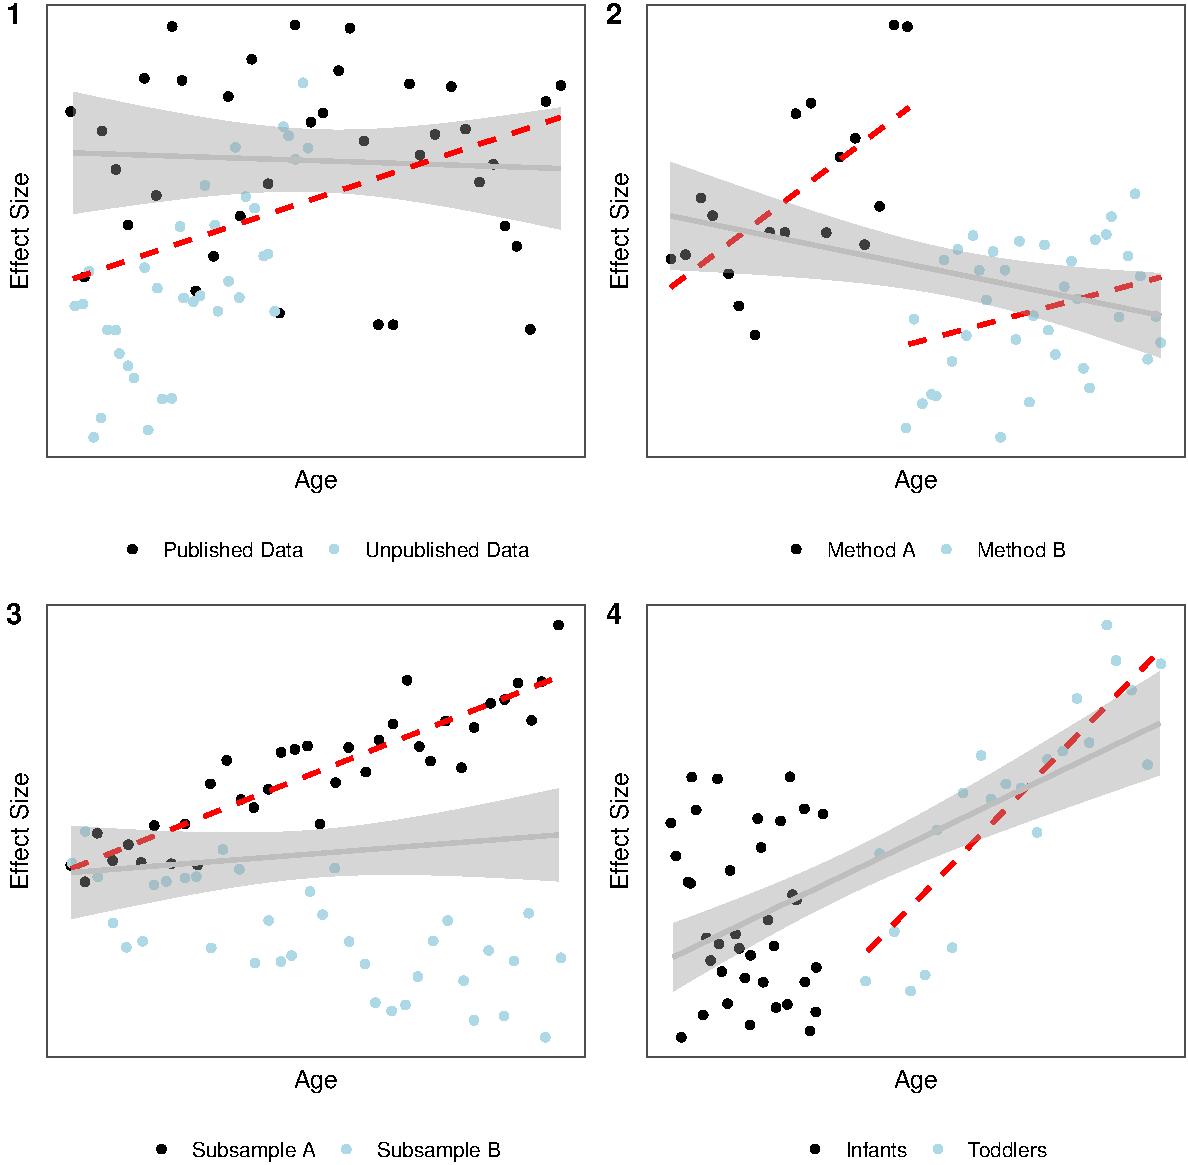
\includegraphics{00_main_files/figure-latex/unnamed-chunk-28-1.pdf}
\caption{\label{fig:unnamed-chunk-28}Schematic illustration of the four hypotheses considered. The gray shaded line represents the observed age effect if the hypothesis holds. The red dotted lines represents the true underlying age effect under the particular hypothesis.}
\end{figure}

\hypertarget{understanding-the-lack-of-developmental-change-in-meta-analytic-data}{%
\section{Understanding the lack of developmental change in meta-analytic data}\label{understanding-the-lack-of-developmental-change-in-meta-analytic-data}}

\hypertarget{age-related-selection-bias-against-younger-infants}{%
\subsection{Age-related selection bias against younger infants}\label{age-related-selection-bias-against-younger-infants}}

We first consider whether age-related selection bias can explain the lack of developmental changes in our datasets. If studies with younger infants suffered from publication bias more, then their effect sizes would be more inflated, obscuring possible developmental changes.

\hypertarget{methods-1}{%
\subsubsection{Methods}\label{methods-1}}

There are many methods to detect publication bias. One of the most common approaches is Egger's test (Egger, Smith, Schneider, \& Minder, 1997), which examines the relationship between the studies' effect sizes and their precision. A significant result from Egger's test indicated an asymmetry in the funnel plot, suggesting the presence of publication bias. This method is more sensitive than the rank correlation approach, another common publication bias detection method (Begg \& Mazumdar, 1994). However, Egger's test can not accommodate predictors other than the study's precision. As a result, we also turned to the weight-function model developed by Vevea and Hedges (1995). This method detects publication bias by likelihood ratio tests: a bias-corrected model is pitted against the original model to see if the former provides a better fit than the latter. A positive result indicates the presence of publication bias.

To detect age-related publication bias, we split each dataset by the median of the average participant age associated with each effect size (in months). We then run both Egger's test and the weight-function model on each half of the dataset. We compared the test outcomes from both tests across the two halves of the datasets. For Egger's test, we used the \texttt{regtest} function implemented in \texttt{metafor} (Viechtbauer, 2010). For the weight-function model, we used the package \texttt{weightr} (Kathleen M. Coburn \& Vevea, 2019) and specified random-effect meta-regression models predicting effect sizes with mean age in months.

\hypertarget{results-and-discussion}{%
\subsubsection{Results and discussion}\label{results-and-discussion}}

Egger's test was run on all but the 4 datasets in which either half of the datasets contained less than 20 effect sizes. Previous study has shown that Egger's test has reduced sensitivity in datasets with less than 20 studies (Sterne, Egger, \& Smith, 2001). For similar reasons, 7 datasets were excluded in the weight-function analysis.

Egger's test suggested that in 3 datasets there was evidence for publication bias in the younger half but not in the older half (\emph{Audio-Visual Congruence}, \emph{Categorization bias}, \emph{Syntactic bootstrapping}). However, this result was not corroborated by the weight-function analysis. For these three datasets, the weight function analysis did not find evidence for publication bias in either half of the three datasets. This suggests that the significant results found by Egger's test might be due to factors other than publication bias. The weight-function analysis did find evidence for publication bias in the younger half but not the older half in two datasets: \emph{Mutual exclusivity} (Younger: \(\chi^2\) = 11.07, \emph{p} \textless{} 0.01; Older: \(\chi^2\) = 0.02, \emph{p} = 0.89) and \emph{Vowel discrimination (non-native)} (Younger: \(\chi^2\) = 5.18, \emph{p} = 0.02; Older: \(\chi^2\) = 1.88, \emph{p} = 0.17). These two datasets yielded significant results for both halves in Egger's test.

Overall, we found little evidence for more severe publication bias among the younger infants. The Egger's test and the function-weight analysis did not yield converging evidence, suggesting that factors other than publication bias may be at play in contributing to the results. Interestingly, out of the five datasets that yield significant results for the younger participants, only \emph{Mutual Exclusivity} originally showed significant age-related changes (\(\beta\) = 0.04, \emph{SE} = 0.01, \emph{z} = 6.01, \emph{p} \textless{} 0.01), which was in contrast with the other three datasets in which the age estimates were trending at the negative direction (\emph{Audio-Visual Congruence}: \(\beta\) = -0.02, \emph{p} = 0.39; \emph{Syntactic bootstrapping}: \(\beta\) = -0.01, \emph{p} = 0.13; \emph{Vowel discrimination (non-native)}: \(\beta\) = -0.01, \emph{p} = 0.45). Taken together, we found some evidence that selective publication bias explains the lack of age-related change across the board.

\hypertarget{methodological-adaptation-for-older-infants}{%
\subsection{Methodological adaptation for older infants}\label{methodological-adaptation-for-older-infants}}

In experiments with young children, many design decisions are made to ensure the paradigms are age appropriate (Byers-Heinlein, Bergmann, \& Savalei, 2022). For older children, more behavioral measures are available and longer experiments are made possible by increased attention span. As a result, experimenters might test more subtle experimental contrasts. Perhaps the increasing difficulty or subtlety of experimental conditions for older infants mask age-related increase in effect sizes related to a particular construct. For example, imagine that different experimenters wanted to study word learning with 12- and 24-month-olds. The experimenter working with the younger group might choose a paradigm in which only two novel words were taught, while the experimenter working with the older children might choose to teach four. The resulting effect for older children might be weaker despite overall improvement in the underlying construct.

The accessibility of different methods could also potentially cause an instance of Simpson's paradox (Kievit et al., 2013). Imagine there were two methods, method A and method B, with the former having lower task demands than the latter. Due to its low task demands, method A would be more likely to be used on younger infants and causes larger effect sizes. In contrast, method B would be more likely to be used on older infants and results in smaller effect sizes. Although the age trend could be positive within each method, when pooling across studies from the two methods, the trend would then be negative, canceling out age-related changes patterns.

Since it is difficult to code for task demands across all studies, we explore whether methodological adaptation influences the developmental trend from the other side: instead of looking at method adaptation with age, we focus on studies using identical methods to test multiple age groups. This subset of datasets should provide the best chance of detecting age-related changes in the absence of methodological variation.

\hypertarget{methods-2}{%
\subsection{Methods}\label{methods-2}}

We first needed to identify the subset of studies in each dataset that satisfy the following two criteria: (1) the same paper tested multiple age groups, and (2) the multiple age groups were all tested using the same experimental design and measure. The first criterion was operationalized as having a paper with multiple age groups with an age difference greater than one month. The second criterion was operationalized based on methodological moderators coded by the original authors and available in MetaLab.

Within the effects selected for each dataset, we calculated \(\Delta_{age}\) for each effect size. \(\Delta_{age}\) was the difference between the age associated with a particular effect size and the minimum age in each subset of the dataset.

19 datasets had subsets of studies fitting our criteria. We focused on the 15 subsets that having 10 and more effect sizes. For each subset, we applied a multilevel meta-regression model using the same nested random intercept as previously described. The model predicts effect sizes based on \(\Delta_{age}\). This analysis follows the logic that, if on average there is a greater effect size when the same experiment is conducted with older children relative to younger children, then the relation of effect size to \(\Delta_{age}\) should be positive.

\hypertarget{results-and-discussion-1}{%
\subsection{Results and discussion}\label{results-and-discussion-1}}

We found no significant relationship between \(\Delta_{age}\) and the effect sizes in any of the dataset (all \emph{p} \textgreater{} 0.05).

This analysis was necessarily constrained by the granularities of the coded moderators. The number of coded methodological moderators ranged from 1 to 9, which means that the experimental design needs to be reduced into at maximum 9 dimensions. However, even at 9 dimensions, it is possible that elements of experiment design influencing task demands were overlooked. For instance, in many domains that use visual stimuli, the particular choice of visual stimuli might significantly vary in complexity (e.g. Cao \& Lewis, 2022). Visual complexity has long been proposed as a key factor influencing the task demands (Hunter \& Ames, 1988), but stimulus complexity was not coded in any of our meta-analyses. In conclusion, the findings presented here should be interpreted with caution due to potential limitations in the coding of methodological moderators.

\hypertarget{change-in-only-a-subsest-of-conditions}{%
\subsection{Change in only a subsest of conditions}\label{change-in-only-a-subsest-of-conditions}}

Across the 25 datasets, 22 datasets were published through manuscripts in peer-reviewed venues Among these manuscripts, we found that 8 papers reported that the meta-analytic effect was significantly stronger in a subset of the data. The subset was often identified by a particular condition in the experimental paradigm (e.g.~experiment that shows ``giving and taking action'' to infants, Margoni \& Surian, 2018), or certain characteristics of the participants (e.g.~bilingual infants, Tsui, Byers-Heinlein, \& Fennell, 2019). In the rest of the data, the meta-analytic effect was either significantly weaker or not present at all. There are many reasons for why the effect would be stronger or only present in a subset of the data. Here, we remain agnostic to the underlying causes for these differences, and leverage these findings to ask: Is it possible that the influence of age was only observable in the subset of the dataset characterized by stronger effect sizes? Perhaps noise in other conditions inadvertently masked age-related changes.

\hypertarget{methods-3}{%
\subsubsection{Methods}\label{methods-3}}

We screened through 22 papers and identified 8 papers that reported a stronger effect on subsets of the data. All subsets had more than 10 effect sizes. For datasets reporting more than one subset as having strong effect, we consider each respectively. In sum, 7 datasets produced 9 subsets that showed stronger effects.

We first investigated whether we could reproduce the original patterns, i.e.~the effect sizes in the better halves were indeed stronger than the other halves. We ran the same multilevel meta-regression without any predictor to estimate the meta-analytic effect sizes in each half. Then we ran a Wald test to compare the two estimates by running a fixed-effects meta-regression model predicting effect sizes with the moderator distinguishing the two halves. A significant estimate on the moderator indicates that the meta-analytic effect sizes in both halves are significantly different from one another. We then estimated the slope of the age predictor in a multilevel meta-regression model for each of the subsets with larger effect sizes.

\hypertarget{results-and-discussion-2}{%
\subsubsection{Results and discussion}\label{results-and-discussion-2}}

We did not fully replicate the original findings reported in the original papers: the ``better half'' identified by the original meta-analysis did not produce significantly stronger effects than the rest of the data in many datasets. We did observe a significantly stronger effect in the remaining 3 datasets: For \emph{Prosocial Agents}, there was a stronger effect in experimental paradigms showing infants giving-taking actions compared to the studies showing infants other stimuli (Margoni \& Surian, 2018, \emph{z} = -2.47, \emph{p} = 0.01); For \emph{Statistical Sound Category Learning}, stronger effect was observed in studies using habituation paradigm compared to other paradigms (Cristia, 2018, \emph{z} = -2.42, \emph{p} = 0.02), and for \emph{Statistical word segmentation}, stronger effect was observed in studies labeled as the conceptual replication of the original work (Black \& Bergmann, 2017, \emph{z} = 2.51, \emph{p} = 0.01).

In addition, we did not find constraining our analyses to the ``better half'' increased the number of significant slope estimates. The two significant slope estimates came from \emph{Mutual Exclusivity} (\(\beta\) = 0.04, \emph{SE} = 0.01, \emph{z} = 4.63, \emph{p} \textless{} 0.01) and \emph{Statistical sound category learning} (\(\beta\) = 0.11, \emph{SE} = 0.05, \emph{z} = 2.23, \emph{p} = 0.03), which also showed significant slopes in the analyses with the full datasets. Qualitatively, we did see that the estimates increased in magnitude in \emph{Syntactic bootstrapping} (\(\beta\) = 0.01, \emph{p} = 0.67) and \emph{Switch task} (\(\beta\) = 0.01, \emph{p} = 0.79), but neither reached the statistical significance threshold.

The discrepancy between our analyses and the previously reported finding suggested that the ``better half effect'' might not be sufficiently robust. This discrepancy could be attributed to the different statistical models we chose -- in the original meta-analysis papers, the models tend to differ in their particular specification of the nested random effect structure and/or in the inclusions of moderators. We chose the simplest model with the maximum random effect structure per recommendation (Barr, Levy, Scheepers, \& Tily, 2013). This approach ensured fair comparison across all datasets, but it could diminish the strength of the reported effects.

Interestingly, even in the datasets where the better half effect was reproduced, we failed to see a significant age effect in the same datasets (Prosocial agents and Statistical word segmentation) that did not show age-related changes in the original full dataset. Altogether, this set of analysis suggested that the theoretical constraints on the effect sizes could not adequately explain the lack of age-related change.

\hypertarget{positive-growth-only-after-infancy}{%
\subsection{Positive growth only after infancy}\label{positive-growth-only-after-infancy}}

Last but not least, we consider whether there is evidence for discontinuity between the growth patterns in infancy and beyond. Bergelson (2020)'s hypothesis on the development of word comprehension suggests a notable shift post the 12-month mark in infancy. This raises the question of whether such distinctions extend across various tasks. This section aims to delve into these dynamics by only looking at the subset of the dataset with infants older than 12-month-olds.

\hypertarget{methods-4}{%
\subsubsection{Methods}\label{methods-4}}

Similar to previous analyses, we filtered each dataset to include only studies that reported more than 10 effect sizes that tested infants older than 12 months. 15 datasets met the criteria. We ran the same meta-regressions predicting effect size with mean age in months on this subset, and then we compared the estimates on the age predictor with the same models run on the full datasets.

\hypertarget{results-and-discussion-3}{%
\subsubsection{Results and discussion}\label{results-and-discussion-3}}

If the discontinuity account is true, we should expect to see more significant age effects to emerge on models run on the subset of data with older infants. We found support for this hypothesis in two datasets, \emph{Cross-situational Word Learning} (\(\beta\) = 0.01, \emph{SE} \textless{} 0.01, \emph{z} = 2.71, \emph{p} = 0.01) and \emph{Mispronunciation sensitivity} (\(\beta\) = 0.07, \emph{SE} = 0.01, \emph{z} = 4.69, \emph{p} \textless{} 0.01). In both datasets, there were no age effects in the full datasets, but significant age-related change in the subsets with older infants. However, we also found the opposite patterns. In \emph{Categorization bias} and \emph{Sound symbolism}, there was evidence for age-related change across the entire age range, but no evidence for age-related change in the toddler subset (Both \emph{p} \textgreater{} 0.05).

\hypertarget{general-discussion}{%
\section{General discussion}\label{general-discussion}}

How do infants' cognitive and linguistic abilities change with age? In this work, we leveraged a dataset of meta-analyses to evaluate the assumption that these abilities increase positively with age, and that the form of this increase is linear. There was no evidence for linear growth in 16 datasets, and interestingly, in all of these datasets, there was no evidence for any age-related growth at all. In the second section, we investigated four potential explanations for this pattern: (1) age-related selection bias against younger infants; (2) methodological adaptation for older infants; (3) change in only a subset of conditions; and (4) positive growth only after infancy.

Our current work has several limitations. First and foremost, we simply lacked sufficient data to investigate the possible explanations for many domains (see Table 3). In many datasets, when we filtered datasets to answer the corresponding questions, we lacked sufficient data to adequately test our hypotheses. Furthermore, as with many meta-analyses, our datasets also had high heterogeneity, meaning that we can only explain relatively small amounts of the variation among effect sizes (see Table 1).

Our work highlights the importance of improving reporting standards in developmental psychology. Testing moderation of heterogeneity requires consistent coding of moderators across datasets. But surveys of reporting standards show that many potential moderators go unreported. For instance, fewer than half of papers report attrition rate (Nicholson et al., 2017; Raad, Bellinger, McCormick, Roberts, \& Steele, 2007). Given these observations, there is a clear need for the developmental psychology community to create and embrace more rigorous and transparent reporting standards. The recently developed framework for reporting demographics information across cultures in developmental psychology is one promising direction moving forwards (Singh et al., 2023). Learning from other fields could provide valuable insights into how to enhance these standards. In biomedical research, numerous reporting standards have been published and widely adopted (for clinical trials: CONSORT, Schulz, Altman, \& Moher, 2010; for epidemiological research: STROBE, Vandenbroucke et al., 2007; for meta-analysis and systematic review, PRISMA: Moher et al., 2015; for a catalog of reporting guidelines in health research: EQUATOR, Altman, Simera, Hoey, Moher, \& Schulz, 2008). Following these structured guidelines in reporting could significantly increase both the quality and the quantity of information extractable from the original papers, providing more traction for tackling heterogeneity in meta-analysis.

Our work also underscores the importance of multi-laboratory large scale replication projects. The relationship between meta-analysis and multi-laboratory is complicated (Kvarven, Strømland, \& Johannesson, 2020; Lewis, Mathur, VanderWeele, \& Frank, 2022). Although the latter approach is much more time- and resource- intensive than the former, it is also much more effective in controlling unwanted heterogeneity and detecting subtle patterns in the data. One prominent example is the comparison between the meta-analysis of Infant directed speech preference (Dunst, Gorman, \& Hamby, 2012) and the ManyBabies 1 project on the same topic (Consortium, 2020). Zettersten et al. (2023) found that, after an update to the meta-analysis dataset, both datasets yielded comparable estimated effect sizes (\emph{d} = 0.35), but the age effect was only detected in the MB1 project, not the meta-analysis. That study speculated that our second explanation (methodological variation covarying with age) might account for their studies. In our analysis, we did investigate the methodological adaptation hypothesis in the IDS preference dataset. However, the methodological moderators available for us were limited and we could not incorporate the varying nature of the stimuli into our analysis. This example shows the potential limitations of meta-analyses that rely on aggregated data from studies with varied methodologies. In contrast, multi-laboratory collaboration projects like Manybabies (Visser et al., 2022) can rely on standardized data collection procedure and stimuli, therefore providing a more controlled dataset to answer a specific research question with high power.

It is also worth considering whether the strengths of certain developmental phenomena truly stay constant throughout the first years of life. First of all, this counterintuitive possibility casts doubts on the construct validity of the existing measures. Many researchers strive to build on existing experimental procedures and measurements when they are testing older participants. This then leads to a potentially problematic situation: an experimental paradigm could have high construct validity with participants of a certain age, but low construct validity with participants of different age. As a result, this leads to an interesting conundrum: methodological adaptation could be a source of significant heterogeneity, diminishing the measurable developmental change. But at the same time, paradoxically, it could also be the prerequisite for properly measuring developmental change. Furthermore, an alternative explanation for the lack of developmental change is the limited sensitivity of cross-sectional design. The group average may stay constant, but there could still be growth in an individual's performance across development (Bornstein, Putnick, \& Esposito, 2017). The nuanced nature of developmental change might be best captured by dense, longitudinal data of individual child (e.g. Bergelson et al., 2023; Sullivan, Mei, Perfors, Wojcik, \& Frank, 2021).

In sum, our current work presents a surprising finding concerning age-related change in the cognitive and language development literatures in early childhood. Despite decades of research built upon the positive increase and linearity assumptions, we failed to find evidence supporting either in most meta-analyses that we had access to. Our work is not intended to overturn the longstanding developmental theories. Like other researchers, we believe that infants get better across different cognitive and linguistic domains as they get older. Instead, our work aims to highlight the needs for more robust reporting standards and more large-scale multi-laboratory projects that measure children consistently across age groups and over time. Our findings invite the cognitive development community to strengthen our understanding of foundational assumptions via collaborative efforts.

\newpage

\hypertarget{references}{%
\section{References}\label{references}}

\hypertarget{refs}{}
\begin{CSLReferences}{1}{0}
\leavevmode\vadjust pre{\hypertarget{ref-adolph2008shape}{}}%
Adolph, K. E., Robinson, S. R., Young, J. W., \& Gill-Alvarez, F. (2008). What is the shape of developmental change? \emph{Psychological Review}, \emph{115}(3), 527.

\leavevmode\vadjust pre{\hypertarget{ref-ahmed2021preschool}{}}%
Ahmed, S. F., Kuhfeld, M., Watts, T. W., Davis-Kean, P. E., \& Vandell, D. L. (2021). Preschool executive function and adult outcomes: A developmental cascade model. \emph{Developmental Psychology}, \emph{57}(12), 2234.

\leavevmode\vadjust pre{\hypertarget{ref-altman2008equator}{}}%
Altman, D. G., Simera, I., Hoey, J., Moher, D., \& Schulz, K. (2008). EQUATOR: Reporting guidelines for health research. \emph{The Lancet}, \emph{371}(9619), 1149--1150.

\leavevmode\vadjust pre{\hypertarget{ref-barr2013random}{}}%
Barr, D. J., Levy, R., Scheepers, C., \& Tily, H. J. (2013). Random effects structure for confirmatory hypothesis testing: Keep it maximal. \emph{Journal of Memory and Language}, \emph{68}(3), 255--278.

\leavevmode\vadjust pre{\hypertarget{ref-begg1994operating}{}}%
Begg, C. B., \& Mazumdar, M. (1994). Operating characteristics of a rank correlation test for publication bias. \emph{Biometrics}, 1088--1101.

\leavevmode\vadjust pre{\hypertarget{ref-bergelson2020comprehension}{}}%
Bergelson, E. (2020). The comprehension boost in early word learning: Older infants are better learners. \emph{Child Development Perspectives}, \emph{14}(3), 142--149.

\leavevmode\vadjust pre{\hypertarget{ref-bergelson2023everyday}{}}%
Bergelson, E., Soderstrom, M., Schwarz, I.-C., Rowland, C. F., Ramirez-Esparza, N., Hamrick, L. R., et al.others. (2023). \emph{Everyday language input and production in 1001 children from 6 continents}.

\leavevmode\vadjust pre{\hypertarget{ref-bergmann2018promoting}{}}%
Bergmann, C., Tsuji, S., Piccinini, P. E., Lewis, M. L., Braginsky, M., Frank, M. C., \& Cristia, A. (2018). Promoting replicability in developmental research through meta-analyses: Insights from language acquisition research. \emph{Child Development}, \emph{89}(6), 1996--2009.

\leavevmode\vadjust pre{\hypertarget{ref-best2015age}{}}%
Best, R., \& Charness, N. (2015). Age differences in the effect of framing on risky choice: A meta-analysis. \emph{Psychology and Aging}, \emph{30}(3), 688.

\leavevmode\vadjust pre{\hypertarget{ref-black2017quantifying}{}}%
Black, A., \& Bergmann, C. (2017). Quantifying infants' statistical word segmentation: A meta-analysis. \emph{39th Annual Meeting of the Cognitive Science Society}, 124--129. Cognitive Science Society.

\leavevmode\vadjust pre{\hypertarget{ref-borenstein2021introduction}{}}%
Borenstein, M., Hedges, L. V., Higgins, J. P., \& Rothstein, H. R. (2021). \emph{Introduction to meta-analysis}. John Wiley \& Sons.

\leavevmode\vadjust pre{\hypertarget{ref-bornstein2018stability}{}}%
Bornstein, M. H., Hahn, C.-S., Putnick, D. L., \& Pearson, R. M. (2018). Stability of core language skill from infancy to adolescence in typical and atypical development. \emph{Science Advances}, \emph{4}(11), eaat7422.

\leavevmode\vadjust pre{\hypertarget{ref-bornstein2017continuity}{}}%
Bornstein, M. H., Putnick, D. L., \& Esposito, G. (2017). Continuity and stability in development. \emph{Child Development Perspectives}, \emph{11}(2), 113--119.

\leavevmode\vadjust pre{\hypertarget{ref-bronfenbrenner1977toward}{}}%
Bronfenbrenner, U. (1977). Toward an experimental ecology of human development. \emph{American Psychologist}, \emph{32}(7), 513.

\leavevmode\vadjust pre{\hypertarget{ref-burnham2004multimodel}{}}%
Burnham, K. P., \& Anderson, D. R. (2004). Multimodel inference: Understanding AIC and BIC in model selection. \emph{Sociological Methods \& Research}, \emph{33}(2), 261--304.

\leavevmode\vadjust pre{\hypertarget{ref-byers2022six}{}}%
Byers-Heinlein, K., Bergmann, C., \& Savalei, V. (2022). Six solutions for more reliable infant research. \emph{Infant and Child Development}, \emph{31}(5), e2296.

\leavevmode\vadjust pre{\hypertarget{ref-cao2022quantifying}{}}%
Cao, A., \& Lewis, M. (2022). Quantifying the syntactic bootstrapping effect in verb learning: A meta-analytic synthesis. \emph{Developmental Science}, \emph{25}(2), e13176.

\leavevmode\vadjust pre{\hypertarget{ref-cao2023synthesis}{}}%
Cao, A., Lewis, M., \& Frank, M. C. (2023). A synthesis of early cognitive and language development using (meta-) meta-analysis. \emph{Proceedings of the Annual Meeting of the Cognitive Science Society}, \emph{45}.

\leavevmode\vadjust pre{\hypertarget{ref-carbajal2021meta}{}}%
Carbajal, M. J., Peperkamp, S., \& Tsuji, S. (2021). A meta-analysis of infants' word-form recognition. \emph{Infancy}, \emph{26}(3), 369--387.

\leavevmode\vadjust pre{\hypertarget{ref-carey2009origin}{}}%
Carey, S. (2009). \emph{The origin of concepts}. Oxford University Press.

\leavevmode\vadjust pre{\hypertarget{ref-coburn2015publication}{}}%
Coburn, Kathleen M., \& Vevea, J. L. (2015). Publication bias as a function of study characteristics. \emph{Psychological Methods}, \emph{20}(3), 310.

\leavevmode\vadjust pre{\hypertarget{ref-weightr2019coburn}{}}%
Coburn, Kathleen M., \& Vevea, J. L. (2019). \emph{Weightr: Estimating weight-function models for publication bias}.

\leavevmode\vadjust pre{\hypertarget{ref-cole2020development}{}}%
Cole, P. M., Lougheed, J. P., Chow, S.-M., \& Ram, N. (2020). Development of emotion regulation dynamics across early childhood: A multiple time-scale approach. \emph{Affective Science}, \emph{1}, 28--41.

\leavevmode\vadjust pre{\hypertarget{ref-manybabies2020quantifying}{}}%
Consortium, M. (2020). Quantifying sources of variability in infancy research using the infant-directed-speech preference. \emph{Advances in Methods and Practices in Psychological Science}, \emph{3}(1), 24--52.

\leavevmode\vadjust pre{\hypertarget{ref-cristia2018can}{}}%
Cristia, A. (2018). Can infants learn phonology in the lab? A meta-analytic answer. \emph{Cognition}, \emph{170}, 312--327.

\leavevmode\vadjust pre{\hypertarget{ref-doebel2015meta}{}}%
Doebel, S., \& Zelazo, P. D. (2015). A meta-analysis of the dimensional change card sort: Implications for developmental theories and the measurement of executive function in children. \emph{Developmental Review}, \emph{38}, 241--268.

\leavevmode\vadjust pre{\hypertarget{ref-dunst2012preference}{}}%
Dunst, C., Gorman, E., \& Hamby, D. (2012). Preference for infant-directed speech in preverbal young children. \emph{Center for Early Literacy Learning}, \emph{5}(1), 1--13.

\leavevmode\vadjust pre{\hypertarget{ref-egger1997meta}{}}%
Egger, M., Smith, G. D., \& Phillips, A. N. (1997). Meta-analysis: Principles and procedures. \emph{Bmj}, \emph{315}(7121), 1533--1537.

\leavevmode\vadjust pre{\hypertarget{ref-egger1997bias}{}}%
Egger, M., Smith, G. D., Schneider, M., \& Minder, C. (1997). Bias in meta-analysis detected by a simple, graphical test. \emph{Bmj}, \emph{315}(7109), 629--634.

\leavevmode\vadjust pre{\hypertarget{ref-elman1996rethinking}{}}%
Elman, J. L. (1996). \emph{Rethinking innateness: A connectionist perspective on development} (Vol. 10). MIT press.

\leavevmode\vadjust pre{\hypertarget{ref-ferguson2012publication}{}}%
Ferguson, C. J., \& Brannick, M. T. (2012). Publication bias in psychological science: Prevalence, methods for identifying and controlling, and implications for the use of meta-analyses. \emph{Psychological Methods}, \emph{17}(1), 120.

\leavevmode\vadjust pre{\hypertarget{ref-ferguson2012vast}{}}%
Ferguson, C. J., \& Heene, M. (2012). A vast graveyard of undead theories: Publication bias and psychological science's aversion to the null. \emph{Perspectives on Psychological Science}, \emph{7}(6), 555--561.

\leavevmode\vadjust pre{\hypertarget{ref-flavell1994cognitive}{}}%
Flavell, J. H. (1994). \emph{Cognitive development: Past, present, and future.}

\leavevmode\vadjust pre{\hypertarget{ref-fletcher2007heterogeneity}{}}%
Fletcher, J. (2007). What is heterogeneity and is it important? \emph{Bmj}, \emph{334}(7584), 94--96.

\leavevmode\vadjust pre{\hypertarget{ref-francis2012publication}{}}%
Francis, G. (2012). Publication bias and the failure of replication in experimental psychology. \emph{Psychonomic Bulletin \& Review}, \emph{19}, 975--991.

\leavevmode\vadjust pre{\hypertarget{ref-frank2017collaborative}{}}%
Frank, M. C., Bergelson, E., Bergmann, C., Cristia, A., Floccia, C., Gervain, J., et al.others. (2017). A collaborative approach to infant research: Promoting reproducibility, best practices, and theory-building. \emph{Infancy}, \emph{22}(4), 421--435.

\leavevmode\vadjust pre{\hypertarget{ref-frank2021variability}{}}%
Frank, M. C., Braginsky, M., Yurovsky, D., \& Marchman, V. A. (2021). \emph{Variability and consistency in early language learning: The wordbank project}. MIT Press.

\leavevmode\vadjust pre{\hypertarget{ref-gasparini2021quantifying}{}}%
Gasparini, L., Langus, A., Tsuji, S., \& Boll-Avetisyan, N. (2021). Quantifying the role of rhythm in infants' language discrimination abilities: A meta-analysis. \emph{Cognition}, \emph{213}, 104757.

\leavevmode\vadjust pre{\hypertarget{ref-higgins2002quantifying}{}}%
Higgins, J. P., \& Thompson, S. G. (2002). Quantifying heterogeneity in a meta-analysis. \emph{Statistics in Medicine}, \emph{21}(11), 1539--1558.

\leavevmode\vadjust pre{\hypertarget{ref-huedo2006assessing}{}}%
Huedo-Medina, T. B., Sánchez-Meca, J., Marı́n-Martı́nez, F., \& Botella, J. (2006). Assessing heterogeneity in meta-analysis: Q statistic or i\(^2\) index? \emph{Psychological Methods}, \emph{11}(2), 193.

\leavevmode\vadjust pre{\hypertarget{ref-hunter1988multifactor}{}}%
Hunter, M. A., \& Ames, E. W. (1988). A multifactor model of infant preferences for novel and familiar stimuli. \emph{Advances in Infancy Research}.

\leavevmode\vadjust pre{\hypertarget{ref-hyde1984large}{}}%
Hyde, J. S. (1984). How large are gender differences in aggression? A developmental meta-analysis. \emph{Developmental Psychology}, \emph{20}(4), 722.

\leavevmode\vadjust pre{\hypertarget{ref-johansson2016individual}{}}%
Johansson, M., Marciszko, C., Brocki, K., \& Bohlin, G. (2016). Individual differences in early executive functions: A longitudinal study from 12 to 36 months. \emph{Infant and Child Development}, \emph{25}(6), 533--549.

\leavevmode\vadjust pre{\hypertarget{ref-karlberg1987analysis}{}}%
Karlberg, J., Engström, I., Karlberg, P., \& Fryer, J. G. (1987). Analysis of linear growth using a mathematical model: I. From birth to three years. \emph{Acta Paediatrica}, \emph{76}(3), 478--488.

\leavevmode\vadjust pre{\hypertarget{ref-kievit2013simpson}{}}%
Kievit, R., Frankenhuis, W. E., Waldorp, L., \& Borsboom, D. (2013). Simpson's paradox in psychological science: A practical guide. \emph{Frontiers in Psychology}, \emph{4}, 54928.

\leavevmode\vadjust pre{\hypertarget{ref-kvarven2020comparing}{}}%
Kvarven, A., Strømland, E., \& Johannesson, M. (2020). Comparing meta-analyses and preregistered multiple-laboratory replication projects. \emph{Nature Human Behaviour}, \emph{4}(4), 423--434.

\leavevmode\vadjust pre{\hypertarget{ref-letourneau2013socioeconomic}{}}%
Letourneau, N. L., Duffett-Leger, L., Levac, L., Watson, B., \& Young-Morris, C. (2013). Socioeconomic status and child development: A meta-analysis. \emph{Journal of Emotional and Behavioral Disorders}, \emph{21}(3), 211--224.

\leavevmode\vadjust pre{\hypertarget{ref-lewis2016quantitative}{}}%
Lewis, M., Braginsky, M., Tsuji, S., Bergmann, C., Piccinini, P. E., Cristia, A., et al. (2016). \emph{A quantitative synthesis of early language acquisition using meta-analysis}.

\leavevmode\vadjust pre{\hypertarget{ref-lewis2022puzzling}{}}%
Lewis, M., Mathur, M. B., VanderWeele, T. J., \& Frank, M. C. (2022). The puzzling relationship between multi-laboratory replications and meta-analyses of the published literature. \emph{Royal Society Open Science}, \emph{9}(2), 211499.

\leavevmode\vadjust pre{\hypertarget{ref-lindenberger1998complex}{}}%
Lindenberger, U., \& Pötter, U. (1998). The complex nature of unique and shared effects in hierarchical linear regression: Implications for developmental psychology. \emph{Psychological Methods}, \emph{3}(2), 218.

\leavevmode\vadjust pre{\hypertarget{ref-margoni2018infants}{}}%
Margoni, F., \& Surian, L. (2018). Infants' evaluation of prosocial and antisocial agents: A meta-analysis. \emph{Developmental Psychology}, \emph{54}(8), 1445.

\leavevmode\vadjust pre{\hypertarget{ref-markman1988children}{}}%
Markman, E. M., \& Wachtel, G. F. (1988). Children's use of mutual exclusivity to constrain the meanings of words. \emph{Cognitive Psychology}, \emph{20}(2), 121--157.

\leavevmode\vadjust pre{\hypertarget{ref-mcardle2009modeling}{}}%
McArdle, J. J., Grimm, K. J., Hamagami, F., Bowles, R. P., \& Meredith, W. (2009). Modeling life-span growth curves of cognition using longitudinal data with multiple samples and changing scales of measurement. \emph{Psychological Methods}, \emph{14}(2), 126.

\leavevmode\vadjust pre{\hypertarget{ref-mccartney1990growing}{}}%
McCartney, K., Harris, M. J., \& Bernieri, F. (1990). Growing up and growing apart: A developmental meta-analysis of twin studies. \emph{Psychological Bulletin}, \emph{107}(2), 226.

\leavevmode\vadjust pre{\hypertarget{ref-moher2015preferred}{}}%
Moher, D., Shamseer, L., Clarke, M., Ghersi, D., Liberati, A., Petticrew, M., \ldots{} Group, P.-P. (2015). Preferred reporting items for systematic review and meta-analysis protocols (PRISMA-p) 2015 statement. \emph{Systematic Reviews}, \emph{4}, 1--9.

\leavevmode\vadjust pre{\hypertarget{ref-naigles1990children}{}}%
Naigles, L. (1990). Children use syntax to learn verb meanings. \emph{Journal of Child Language}, \emph{17}(2), 357--374.

\leavevmode\vadjust pre{\hypertarget{ref-nicholson2017attrition}{}}%
Nicholson, J. S., Deboeck, P. R., \& Howard, W. (2017). Attrition in developmental psychology: A review of modern missing data reporting and practices. \emph{International Journal of Behavioral Development}, \emph{41}(1), 143--153.

\leavevmode\vadjust pre{\hypertarget{ref-oakes2019developmental}{}}%
Oakes, L. M., \& Rakison, D. H. (2019). \emph{Developmental cascades: Building the infant mind}. Oxford University Press.

\leavevmode\vadjust pre{\hypertarget{ref-piaget1971theory}{}}%
Piaget, J. (1971). \emph{The theory of stages in cognitive development.}

\leavevmode\vadjust pre{\hypertarget{ref-publications2008reporting}{}}%
Publications, A., \& Journal Article Reporting Standards., C. B. W. G. on. (2008). Reporting standards for research in psychology: Why do we need them? What might they be? \emph{The American Psychologist}, \emph{63}(9), 839.

\leavevmode\vadjust pre{\hypertarget{ref-raad2007brief}{}}%
Raad, J. M., Bellinger, S., McCormick, E., Roberts, M. C., \& Steele, R. G. (2007). Brief report: Reporting practices of methodological information in four journals of pediatric and child psychology. \emph{Journal of Pediatric Psychology}, \emph{33}(7), 688--693.

\leavevmode\vadjust pre{\hypertarget{ref-saffran1996statistical}{}}%
Saffran, J. R., Aslin, R. N., \& Newport, E. L. (1996). Statistical learning by 8-month-old infants. \emph{Science}, \emph{274}(5294), 1926--1928.

\leavevmode\vadjust pre{\hypertarget{ref-schulz2010consort}{}}%
Schulz, K. F., Altman, D. G., \& Moher, D. (2010). CONSORT 2010 statement: Updated guidelines for reporting parallel group randomised trials. \emph{Journal of Pharmacology and Pharmacotherapeutics}, \emph{1}(2), 100--107.

\leavevmode\vadjust pre{\hypertarget{ref-simonsohn2022above}{}}%
Simonsohn, U., Simmons, J., \& Nelson, L. D. (2022). Above averaging in literature reviews. \emph{Nature Reviews Psychology}, \emph{1}(10), 551--552.

\leavevmode\vadjust pre{\hypertarget{ref-simpson1951interpretation}{}}%
Simpson, E. H. (1951). The interpretation of interaction in contingency tables. \emph{Journal of the Royal Statistical Society: Series B (Methodological)}, \emph{13}(2), 238--241.

\leavevmode\vadjust pre{\hypertarget{ref-singh2023unified}{}}%
Singh, L., Barokova, M. D., Baumgartner, H. A., Lopera-Perez, D. C., Omane, P. O., Sheskin, M., et al.others. (2023). A unified approach to demographic data collection for research with young children across diverse cultures. \emph{Developmental Psychology}.

\leavevmode\vadjust pre{\hypertarget{ref-sterne2001investigating}{}}%
Sterne, J. A., Egger, M., \& Smith, G. D. (2001). Investigating and dealing with publication and other biases in meta-analysis. \emph{Bmj}, \emph{323}(7304), 101--105.

\leavevmode\vadjust pre{\hypertarget{ref-sugden2017meta}{}}%
Sugden, N. A., \& Marquis, A. R. (2017). Meta-analytic review of the development of face discrimination in infancy: Face race, face gender, infant age, and methodology moderate face discrimination. \emph{Psychological Bulletin}, \emph{143}(11), 1201.

\leavevmode\vadjust pre{\hypertarget{ref-sullivan2021saycam}{}}%
Sullivan, J., Mei, M., Perfors, A., Wojcik, E., \& Frank, M. C. (2021). SAYCam: A large, longitudinal audiovisual dataset recorded from the infant's perspective. \emph{Open Mind}, \emph{5}, 20--29.

\leavevmode\vadjust pre{\hypertarget{ref-thelen2007dynamic}{}}%
Thelen, E., \& Smith, L. B. (2007). Dynamic systems theories. \emph{Handbook of Child Psychology}, \emph{1}.

\leavevmode\vadjust pre{\hypertarget{ref-thompson1999explaining}{}}%
Thompson, S. G., \& Sharp, S. J. (1999). Explaining heterogeneity in meta-analysis: A comparison of methods. \emph{Statistics in Medicine}, \emph{18}(20), 2693--2708.

\leavevmode\vadjust pre{\hypertarget{ref-thornton2000publication}{}}%
Thornton, A., \& Lee, P. (2000). Publication bias in meta-analysis: Its causes and consequences. \emph{Journal of Clinical Epidemiology}, \emph{53}(2), 207--216.

\leavevmode\vadjust pre{\hypertarget{ref-tilling2014modelling}{}}%
Tilling, K., Macdonald-Wallis, C., Lawlor, D. A., Hughes, R. A., \& Howe, L. D. (2014). Modelling childhood growth using fractional polynomials and linear splines. \emph{Annals of Nutrition and Metabolism}, \emph{65}(2-3), 129--138.

\leavevmode\vadjust pre{\hypertarget{ref-tsui2019associative}{}}%
Tsui, A. S. M., Byers-Heinlein, K., \& Fennell, C. T. (2019). Associative word learning in infancy: A meta-analysis of the switch task. \emph{Developmental Psychology}, \emph{55}(5), 934.

\leavevmode\vadjust pre{\hypertarget{ref-vandenbroucke2007strengthening}{}}%
Vandenbroucke, J. P., Elm, E. von, Altman, D. G., Gøtzsche, P. C., Mulrow, C. D., Pocock, S. J., \ldots{} Initiative, S. (2007). Strengthening the reporting of observational studies in epidemiology (STROBE): Explanation and elaboration. \emph{Annals of Internal Medicine}, \emph{147}(8), W--163.

\leavevmode\vadjust pre{\hypertarget{ref-vevea1995general}{}}%
Vevea, J. L., \& Hedges, L. V. (1995). A general linear model for estimating effect size in the presence of publication bias. \emph{Psychometrika}, \emph{60}, 419--435.

\leavevmode\vadjust pre{\hypertarget{ref-viechtbauer2010conducting}{}}%
Viechtbauer, W. (2010). Conducting meta-analyses in r with the metafor package. \emph{Journal of Statistical Software}, \emph{36}(3), 1--48.

\leavevmode\vadjust pre{\hypertarget{ref-visser2022improving}{}}%
Visser, I., Bergmann, C., Byers-Heinlein, K., Dal Ben, R., Duch, W., Forbes, S., et al.others. (2022). Improving the generalizability of infant psychological research: The ManyBabies model. \emph{Behavioral and Brain Sciences}, \emph{45}.

\leavevmode\vadjust pre{\hypertarget{ref-zettersten2023evidence}{}}%
Zettersten, M., Cox, C. M. M., Bergmann, C., Tsui, A., Soderstrom, M., Mayor, J., et al.others. (2023). \emph{Evidence for infant-directed speech preference is consistent across large-scale, multi-site replication and meta-analysis}.

\end{CSLReferences}


\end{document}
